\chapter{Other projects and tools}\label{other_projects}

This chapter presents a few other mention-worthy projects and tools that I worked on during my thesis.

\localtableofcontents

\section{Bacterial chromatin and HU}

Initially the main project of my PhD, the study of bacterial chromatin compaction by cryo-EM and cryo-ET is an ongoing project in the MICA group, which builds upon previous fluorescence imaging done by the GenOM team on \textit{D. radiodurans} nucleoids.
The main protein of interest is HU, a nucleoid-associated protein (NAP) present in many bacteria (including \textit{E. coli} and \textit{D. radiodurans}) which is known to be a key player in chromatin compaction and nucleoid morphology throughout the cell cycle.
The structure of monomeric HU has been solved in multiple occasions (\autoref{fig:hu}), but the literature is inconclusive about the structure of its complex with DNA.
Indeed, while HU is expected to have a histone-like function --- and some molecular dynamics studies support this hypothesis CITE --- other modes of interaction between HU monomers and the DNA have been identified by X-ray crystallography CITE.

\begin{figure}[ht]
    \centering
    \begin{subfigure}[B]{.48\textwidth}
        \centering
        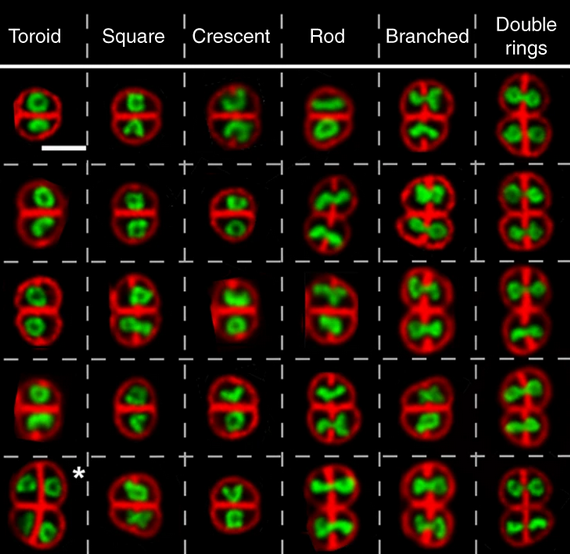
\includegraphics[width=\textwidth]{other/dr_nucleoids.png}
        \caption{\textit{D. radiodurans} heterogeneous and dynamic nucleoid shows variations throughout the cell cycle. Image taken from \citet{flochCellMorphologyNucleoid2019}.}
        \label{fig:hu_nucleoids}
    \end{subfigure}%
    \hfill
    \begin{subfigure}[B]{.5\textwidth}
        \centering
        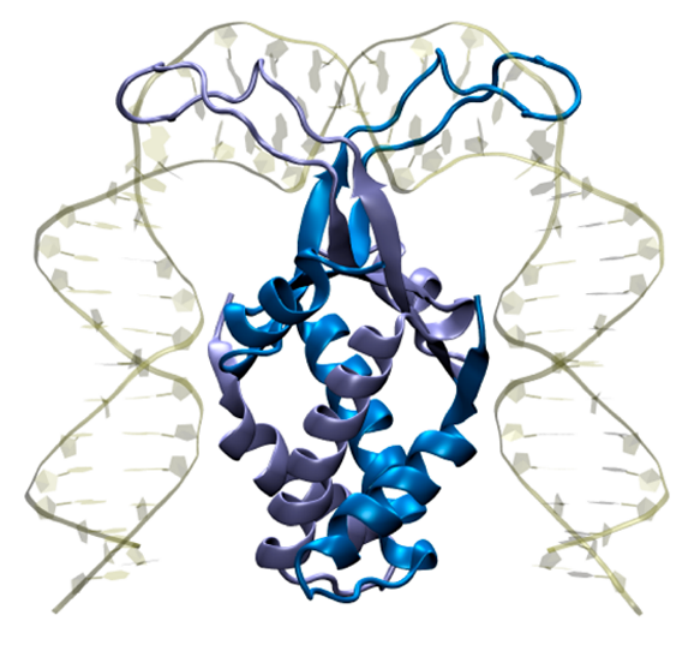
\includegraphics[width=\textwidth]{other/hu_struct.png}
        \caption{\textit{Borrelia burgdorferi} HU showing histon-like behavior in complex with DNA, as predicted by molecular dynamics. Image taken from \citet{hognonMolecularBasesDNA2019}.}
        \label{fig:hu_structure}
    \end{subfigure}%
    \titledcaption[\textit{D. radiodurans} nucleoids and HU structure]{\textbf{(a)} Nucleoid compaction and morphology in \textit{D. radiodurans} is complex and dynamic, with HU being one of the major drivers of chromatin compaction. \textbf{(b)} HU is thought to have a histone-like behaviour, bending the DNA to form a tight kink.}
    \label{fig:hu}
\end{figure}

To begin investigating DrHU in complex with the DNA, we collected single particle cryo-EM data of an \textit{in vitro} preparation of plasmid DNA and HU, in order to observe the interaction in a free acqueous environment.
Within a small range of relative concentrations, intriguing spirals (\autoref{fig:hu_spirals}) were formed by the DNA, suggesting a certain folding was caused by HU.

\begin{figure}[ht]
    \centering
    \includegraphics[width=\textwidth]{other/hu_spirals_no_spirals.png}
    \titledcaption[HU-induced DNA spirals]{Spiral formations of DNA are formed in presence of HU only at specific concentration ranges.}
    \label{fig:hu_spirals}
\end{figure}

The very small molecular weight of HU (\sim12.5 kDa) meant that picking and processing these particles (even in the expected dimeric or tetrameric forms) would be practically impossible in cryo-EM (see \autoref{fig:et_smallest_particle} for the theoretical limits).
However, it should be possible to work around this limitation by using a supporting geometry --- such as the DNA filament --- to do the picking and guide refinement.

This, unfortunately, proved unsuccessful; while we were able to pick and classify on the DNA and several interesting "blobs" next to it (\autoref{fig:hu_classes}), we could never identify them or reach high resolution.

\begin{figure}[ht]
    \centering
    \includegraphics[width=\textwidth]{other/hu_classes.png}
    \titledcaption[HU+DNA: representative 2D classes]{Representative classification results from generic particle picks from the filament picker (top) and from picks centered on "blobs" next to the DNA (bottom).}
    \label{fig:hu_classes}
\end{figure}

Classification and refinement are not only made difficult by the small size of HU, but also by the heterogeneous and dynamic nature of the HU-DNA complex.

\subsection{Future perspectives}

To increase our chances to identify and pick HU, a new dataset was collected with a phase plate, which allows to collect data closer to focus while improving the contrast of low spacial fequency information (\fullref{em_ctf}).

Preliminary results on this data showed more classes containing what could HU in a similar conformation to what seen in \autoref{fig:hu_structure} (\autoref{fig:hu_blobs}).

\begin{figure}[ht]
    \centering
    \includegraphics[width=\textwidth]{other/hu_blobs.png}
    \titledcaption[HU+DNA: promising 2D classes]{Promising 2D classes from the phase plate dataset, potentially showcasing DNA in complex with HU.}
    \label{fig:hu_blobs}
\end{figure}

TODO: some hint on irina's ideas?

\section{waretomo}

As most cryo-ET users, over time I kept tweaking and improving my processing pipeline.
At present, it consists of three main elements: Warp~\cite{tegunovRealtimeCryoelectronMicroscopy2019} for preprocessing and tomogram and subtomogram reconstruction, AreTomo~\cite{zhengAreTomoIntegratedSoftware2022} for tilt series alignment, and Relion~\cite{scheresRELIONImplementationBayesian2012,zivanovBayesianApproachSingleparticle2022,burtImageProcessingPipeline2024} for STA.

To facilitate batch processing and remove most needs for manual intervention (and potential points of failure), I developed an automated tool which connects Warp to AreTomo: \href{https://gihub.com/brisvag/waretomo}{waretomo}~\cite{gaifasWaretomoV02024}.

\section{emscan}

This tool was developed as a contribution to the PhD project of Eymeline Pageot, from the MICA group, under the supervision of Ambroise Desfosses.

\href{https://gihub.com/brisvag/emscan}{emscan}

\section{Teamtomo}

\href{https://teamtomo.org}{teamtomo}
\section{napari tools}
molecular viewer
fourier transform simulator
euler angle playground

\section{Surforama}

\section{cryosparc, cs2star}

\section{stemia}

\subsection{Out-of-plane angle generation}\label{stemia_angles}
This tool was developed to work on the FtsZ tilted dataset (\fullref{ftsz_tilted}).

\begin{outline}
\1 HU...
    \2 initial proposition: bacterial chromatin, connect to Dr chapter
    \2 interesting spiral formations, unexplained, reproducible
    \2 tricky sample preparation, very small protein
        \3 attempts as solving using DNA as scaffolding for picking, etc...
        \3 cryoet proof of concept
\1 teamtomo!
    \2 goal proposition, community efforts
\1 projection matching for eymeline's work
    \2 more native than SPA but more straightforward than STA
    \2 would be cool to go into some technical details here (cross-correlation, projection, etc)
    \2 optimizing for space and performance
    \2 the issues around cross correlation
\1 cs2star and cryosparc in general and related tools
\1 stemia and collection of tools... how to wrap this us in a way that makes sense?
\1 waretomo
    \2 some suites exist that do the "whole" procedure, but they are monolithic and hard to get in/out for special cases, which occurs frequently in cryoet
    \2 difficulties with metadata wrangling
\1 molecular viewer napari
\end{outline}
